\documentclass[]{final_report}
\usepackage{graphicx}
\usepackage{hyperref}
\usepackage{cite}
\usepackage{url}

%%%%%%%%%%%%%%%%%%%%%%
%%% Input project details
\def\studentname{Bjørn Mathias Helseth}
\def\reportyear{2020}
\def\projecttitle{A Dangerous Impasse: Identifying how lightweight statistical tests of randomness fail to identify supply chain threat vectors, and relevant remediation strategies}
\def\smallprojecttitle{A Dangerous Impasse}
\def\supervisorname{Prof. Darren Hurley-Smith}
\def\degree{BSc (Hons) in Computer Science}
\def\fullOrHalfUnit{Full Unit} % indicate if you are doing the project as a Full Unit or Half Unit
\def\finalOrInterim{Interim} % indicate if this document is your Final Report or Interim Report

\begin{document}

\maketitle

%%%%%%%%%%%%%%%%%%%%%%
%%% Declaration

\chapter*{Declaration}

This report has been prepared on the basis of my own work. Where other published and unpublished source materials have been used, these have been acknowledged.

\vskip3em

Word Count: 

\vskip3em

Student Name: \studentname

\vskip3em

Date of Submission: 7th of December 2020

\vskip3em

Signature:
\newline
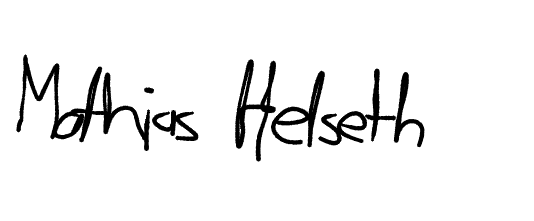
\includegraphics[width=4cm]{signature}

\newpage

%%%%%%%%%%%%%%%%%%%%%%
%%% Table of Contents
\tableofcontents\pdfbookmark[0]{Table of Contents}{toc}\newpage

%%%%%%%%%%%%%%%%%%%%%%
%%% Project Spec or Introduction
\chapter*{Introduction}
\addcontentsline{toc}{chapter}{Introduction}

\section*{Aims}
\addcontentsline{toc}{section}{Aims}
\begin{itemize}
	\item{Exploring how Random Number Generators (RNGs), particularly True RNGs, can be vulnerable in the supply chain against critical security infrastructure attacks}
	\item{Researching remediation strategies against supply chain attacks.}
	\item{Examining test data from various different RNG statistical test suites, with the aim of understanding why some RNGs might pass a test even with trojanised input from an adversary confusing the RNG bias.}
	\item{Develop statistical tests in Python and C (See \nameref{appendixa} for instructions on how to locate the code) to better understand underlying test data and to examine the data in statistical analysis through e.g. MatLab}
\end{itemize}

\section*{Background}
\addcontentsline{toc}{section}{Background}

\par{Random Number Generators (RNGs) are used in various different applications e.g. authentication protocols. Some of these applications therefore needs to be cryptographically secure by design. Statistical tests of randomness can help identify the generators ability or incapability of generating random behaviour through analysis of the RNGs output stream. Different batteries of tests exists to perform such analysis, e.g. NIST SP 800-22/800-90b, Dieharder, TestU01 and - although deprecated - FIPS 140-2. The latter is to be followed by FIPS 140-3.}

\par{Despite deprecated and followed by a newer standard, FIPS 140-2 is still in use. Manufacturers and resellers are still labelling their RNGs with FIPS 140-2 certifications and they are still popular in use as lightweight self-tests of Hardware RNGs (HRNG). However, recent research of the tests provided in FIPS 140-2 have shown that they are not capable to identify tampering or structured information concealed in the generators output stream. These concealments are likely to be trojanised into the HRNG during its transport through e.g. the supply chain or through other channels, such as reselling.}

\par{This project will identify supply chain threat vectors and remediation strategies that are cost-effective and simple, the aim being to identify methods for end-users to independently pinpoint these vectors and strategies in a simple way.}

%%%%%%%%%%%%%%%%%%%%%%
%%% Literature review
\chapter*{Literature Review}
\addcontentsline{toc}{chapter}{Literature Review}

\par{This chapter is dedicated to demonstrate my insight into the project through the research I have done so far. }

\par{While there has been a significant amount of research done on the different statistical test suites and their vulnerabilities, there has been less research dedicated to identifying threat vectors in the supply chain of RNGs and remediation strategies. Therefore, I have focused my project towards this topic. I am interested to see if there has been done research which concludes any of my questions that I raise in my reports as of now.}

\par{In my \nameref{SupplyChainAttacksReport} report, I have found through my research that there could be introduced several different attacks towards TRNGs while they are circulating in the supply chain. In the report I raise several questions as to why the RNGs can't be trusted when received to the end-customer and why we safely can't assume their integrity even when in use. The manufacturer can label their TRNGs with certifications from different test suites. However, after it has left the manufacturer, the generator is vulnerable to trojanising attacks.}

\par{As found in my research so far. The main concern for researchers that have been analysing different statistical test suites, seems to be that the tests fail to discover underlying bias from potential adversaries. This could be a substantial threat to companies and individuals adopting these RNGs into their systems to generate e.g. cryptographic tokens.}

\par{In this project there has been reason to particularly look at two different types of RNGs. True Random Number Generators (TRNGs) and Pseudo-Random Number Generators (PRNGs), where my main area of focus has been TRNGs. While there exists another fraction of TRNGs which extends further than the classical ones, namely Quantum Random Number Generators (QRNGs). I have settled with researching the supply chain of TRNGs which derives from physical processes, such as thermal noise and radioactive decay. The reason being that QRNGs would advance the project out-of-scope.}

\par{For the research I have currently done, there has been focus on researching existing publications on the matter of vulnerabilities against TRNGs in-and-out of the supply chain. To be able to reason about this in this report so far, some tests have been conducted to better understand the underlying factors used in the different batteries of tests found in statistical test suites. For these tests to be conducted, I have been implementing code in C in a UNIX environment to test different TRNGs and also the /urandom and /random generators found in most UNIX distributions.}

\par{The testing up until this point has been mainly focused around understanding the test suites. Further code that can be developed for this project may be used to implement the test in statistical analysis. A couple of the tests found in FIPS 140-2 are simple statistical tests, such as the monobit test, poker-test and runs-test. A simple implementation overview of these tests can be found in this publication of Hurley-Smith et al.\cite{Smith:2020}.}

\par{The reading I have been doing for this report has been varied, as I am looking into both RNGs and the their supply chain. Currently, my supervisor's previous work in this field has been very relevant and multiple citations have been made from his work in this report already. The work of Hotoleanu et al. has also contributed to multiple comments I have made in this report. They acknowledge that a hardware implementation of statistical test suites can be of advantage to the user, as it can be faster and more reliable. However, there were some drawbacks of this implementation, as only 8 out of 14 tests were suitable to hardware implement.\cite{Hotoleanu:2010}}

\newpage
\section*{Hardware Random Number Generators}
\addcontentsline{toc}{section}{Hardware Random Number Generators}

\par{Hardware Random Number Generators (HRNGs) benefits from random events from a physical source in order to generate its entropy pool. The output bit-stream of a HRNG will be non-deterministic and independent and identically distributed, which means that the outcome of each bit in the bit-stream has the same probability distribution. Some examples of HRNGs are the ChaosKey by Altus Metrum and TectroLabs TL200.}

\par{The physical source of randomness in HRNGs can come from various different phenomenas, such as decay of radioactive materials\cite{Rohe:2003}, thermal noise\cite{Rohe:2003} and atmospheric noise\cite{Jun:1999}. As Stipčević et al.\cite{Stipcevic:2014} notes, "Our assumption has been that random numbers cannot be computed; because digital computers operate deterministically, they cannot produce random numbers", therefore we use random numbers generated by a physical hardware generator which is known as a True RNG (TRNG).}

\par{Pseudo-Random Number Generators (PRNGs) on the other hand harvest entropy from software events. As PRNGs relies purely on software implementations and its entropy comes from algorithms rather than actual physical and random events, it is deterministic. As Hurley-Smith et al.\cite{Smith:2018} notes, PRNGs are initialised through seed values. If the seed of a PRNG become known, the output can be predicted.}

\par{HRNGs can also be used as a hybrid generator in conjunction with PRNGs. In this case the HRNG is used as a seed generator for the PRNG. If we want a cryptographically secure PRNG we should have a random initial seed value. A HRNG can provide this. Using the HRNG and a PRNG together as a hybrid solution can create a Cryptographically Secure RNG (CSRNG) which is a subset of PRNGs which are considered secure.}

\par{There are a number of different use cases for RNGs. In cryptographical settings, the need for these to be cryptographically secure can be crucial. Both for the end-user and the manufacturer. One of the use cases is in authentication protocols\cite{Han:2009}. Here the use of unbiased, unpredictable and entropically rich random numbers are essential to provide a safe platform with little-to-no risk that an adversary might be able to decrypt random keys produced and fed into the system for authentication purposes.}

\par{When implementing a hybrid solution into a secure system, a whitening function is normally used to remove non-random components from the output stream\cite{Holleman:2008}. A whitening function can also be used from a TRNGs output as well as the hybrid solution to clean up the output. While there exists a number of different whitening functions, some generally used ones include Von Neumann and XOR operations over the bit-stream output.}

\par{Looking further into how these RNG’s work, it could be possible to establish a sense of how we may analyse their output in a lightweight statistical manner to ensure that we do in fact have a truly random output with no obvious bias or a low entropically filled pool. Can we see a clear difference in what a TRNG and a PRNG are able to output?}

\par{In a PRNG we can find that the entropy pool can fill up or stop being refreshed with new input data. This is often the case that makes PRNGs less cryptographically secure. As well as the problem with PRNGs where, if you know the seed, you can generate or predict new numbers. If we make an assumption that we have the entropy pool in one PRNG fill up with user input (clicks, mouse movement and keystrokes). This can at any point stop being fed new input, and therefore the generator will have to take its inputs from the same entropy pool. This can lead to the generator outputting sequences or simply repeating the same patterns.}

\par{As we can see in Figure \ref{fig:TableA} by Vuillemin et al. \cite{Vuillemin:2012} in the first output table. The proportion of entropy gathered from user input can be substantial to generate PRNG entropy. Running out of entropy in a PRNG is hard, so this should not be a concern. From the two other scenarios in Figure \ref{fig:TableA} where there is no actual user input, the amount of entropy gathered from the disk is increased.}

\begin{figure}[h!]
\begin{center}
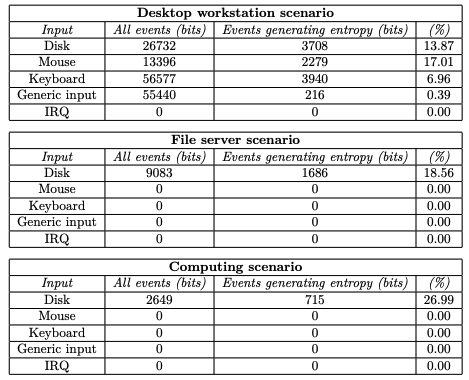
\includegraphics[height=8cm]{TableA}
\caption{Proportion of input events that generate entropy\cite{Vuillemin:2012}}
\label{fig:TableA}
\end{center}
\end{figure}

\par{In a TRNG we usually find different sources of entropy used. These are physical and natural events happening at an unpredictable rate, creating ‘noise’. The most commonly used entropic sources in use for TRNGs as I have found on the market are among others, decay of radioactive materials\cite{Rohe:2003}, thermal noise\cite{Rohe:2003} and atmospheric noise\cite{Jun:1999}. These allow the generator to be fed with constant noise from a source found to be unpredictable.}

\par{Currently, on the market there are a number of different TRNGs that are being sold\footnote{\url{https://www.aliexpress.com/af/TRNG-noise.html} and \url{https://www.amazon.com/TrueRNG-V3-Hardware-Random-Generator/dp/B01KR2JHTA}}, both privately and by corporations manufacturing them. The majority of these TRNGs are marketed as being able to pass all the top industry standard statistical tests such as Dieharder and FIPS 140-2 just to mention some of them. This seems to be their main selling point in addition to their output speed. Now, can we trust these statements without actually testing this ourselves? How can we know that there is actually some cryptographically secure module inside the enclosure of this physical device, that will be able to provide us with such high- level of entropy and randomness?}

\par{These industry standard tests are usually performed by the manufacturer, which provides the results. How can we however know that they haven’t been changed after the tests, can we trust the results ourselves and could someone have tampered with the device before it got to the end user? These are vulnerabilities that can be found in most TRNGs purchased online. Could lightweight statistical tests of randomness be more available to the end-user so this can be tested more efficiently and easily?}

\par{PRNGs are as earlier stated, without a random bias, unsecure. A Cryptographically Secure PRNG (CSPRNG) seeded by a TRNG in a hybrid approach would be superior to a PRNG. If we look into the /dev/urandom function on most Linux distributions. It is provided through user input and other events to fill up the entropy pool. However, what makes /dev/urandom cryptographically less secure than for example /dev/random, is because it does not block the generator from proceeding to output numbers even though its entropy pool is filled up. Which can make up sequences which are repetitive and therefore not random. We can use a third-party TRNG (such as the ChaosKey by Altus Metrum) to fill the pool serving as a seed for urandom or random, making them CSPRNG}

\par{Performing statistical tests of randomness on RNGs can tell us more about the characteristics of the generator in question and can help determine whether or not the RNG is suitable for use in applications as a secure way of deliver randomness. Helping the end-user performing these tests can lead to any adversary to not be able to penetrate an application that could have otherwise been easily intrudable through deterministic randomness.}

\par{Statistical tests of randomness can be used to check a generators ability to produce random numbers out of a set of tests. Tests suites available include, Dieharder and NIST SP 800-22/800-90b. The FIPS 140-2 tests were used as a US government standard to ensure cryptographic security within their applications. This test suite is now becoming deprecated and replaced by FIPS 140-3\cite{NIST:2019}.}

\par{Generation of random numbers through an external physical event, would possibly be the most secure way to generate these random numbers. The reason being that it does not require a seed. Therefore, as it is independently and identically distributed (IID) as well as non-deterministic, it conforms a forward-secrecy model by having the next bit in the sequence non-related to the previous bit. However, the adversary might be able to bias the entropy source to perform with a distribution that is predicted to, for example output numbers with less entropy by moving the entropy source itself. If we assume that these vulnerabilities exist, we can try to find remediation strategies.}

\newpage
\section*{Supply Chain Attacks} 
\label{SupplyChainAttacksReport}
\addcontentsline{toc}{section}{Supply Chain Attacks}

\par{Currently, Random Number Generator (RNG) manufacturers continuously use the statistical tests of randomness found in for example standards such as FIPS 140-2 to prove that their RNG is cryptographically secure. Even though this particular standard for statistical tests is now starting to become deprecated \cite{NIST:2019}, it is still widely used in the supply chain by manufacturers to prove that their RNGs are producing output which can be used in cryptographical applications to provide a secure layer of randomness. How can we know that the claims of the manufacturer stand true at the point it is handed to the end-customer?}

\par{If we assume three phases of the process of distributing Hardware RNGs (HRNGs), just to provide an example of the level of trust signed by the end-customer to the RNG manufacturers. The manufacturing phase, the supply chain and then leaving the supply chain to the end-user or organisation. In these phases, we can assume that there are different vulnerabilities that can be introduced to the RNG in circulation.}

\par{We should be worried about these assumed vulnerabilities being present in the supply chain, so that we can prevent adversarial tampering of the RNGs. If the statistical tests are to be trusted, they should be able to detect adversarial bias. As Hurley-Smith et al. \cite{Smith:2020} states in their journal on the lightness of FIPS 140-2, “Our research shows that FIPS 140-2 cannot identify adversarial biases effectively, even very primitive ones.”. This can lead us to think that this commonly used statistical testing suite, can’t be trusted for use in testing the integrity of an RNG after it has been manufactured.}

\par{For statistical testing of randomness, there are generally a series of tests being performed on n-bit-blocks from the output stream. These tests look for particular distinctive characteristics usually found in random sequences. In the NIST SP800-22 and FIPS 140-2 batteries of tests for example, we find similar \cite{Smith:2020}\cite{Rukhin:2010} tests being used for general testing, such as the monobit test where we test to see if the number of ones and zeroes in a bit-block sequence are approximately the same as in a truly random sequence. However, the batteries usually differ with additional tests than the general ones used in most statistical test suites.}

\par{As stated by Bill Phelps, Commercial Lead in Booz Allen Consulting \cite{Phelps:2019}, increasing the visibility into the supply chain, a good relationship with the suppliers and planning remediation strategies against breaches can help the manufacturer mitigate supply chain attacks. However, in the supply chain there might be imposed attacks by an adversary after it leaves the manufacturer. These attacks could even happen physically towards the RNG creating external bias to the RNGs entropy source. Such as with thermal noise RNGs where noise-based attacks can be executed to create bias \cite{Brown:2020}.}

\par{An adversary may be interested in implementing bias to the RNG, while still making sure that it will be able to pass the most common batteries of statistical tests performed by manufacturers at the point of manufacture, and by the end-customer at the point of usage. However, we can’t safely assume that the customer will be able to perform these software tests on their own as it may require some technical knowledge of RNGs. They can be time consuming to perform and require some background information of the statistical tests in order to understand the results as well.  By implementing a low-cost on-chip hardware layer of lightweight statistical tests that may remove the trivial steps for the consumer, we may be able to mitigate some of the adversarial input.}

\par{On-chip hardware statistical tests could be an addition, but maybe not alternative, to the software-based statistical test batteries that exist today. As Hoţoleanu et al. \cite{Hotoleanu:2010} notes, during their experiment implementing the NIST SP800-22 statistical tests onto a FPGA board. They found that only 8 of the 14 tests\footnote{14 out of the 16 total tests in the NIST SP800-22 were recommended by NIST at the time of their experiment\cite{Hotoleanu:2010}} were suitable for lightweight hardware use. Yang\cite{Yang:2016} also found similar results with a FPGA implementation of NIST tests.}

\par{Having these hardware implemented tests we could introduce new solutions to deal with adversarial analysis of the RNG. By introducing a decontamination protocol for the end-customer, where the RNG is to be placed under a strict test regime during its first entry under new hands. This could help mitigate unexpected/unwanted behaviour in the RNGs by finding potential leaks in the design through statistical testing. This may however not be to any help if the adversarial input bias is well designed, lacks flaws and/or are able to pass the statistical tests.}

\par{Looking at the experiments conducted by Hotoleanu et al.\cite{Hotoleanu:2010} and Yang\cite{Yang:2016} to implement statistical tests in hardware. We have some tests that can be implemented in hardware. and some that can't be due to limitations. Generating a protocol to separate which tests that can be implemented in hardware and which that needs to be implemented in software. it could be possible to define a maximum number of tests needed to execute a given test suite appropriately (or define a new test suite) in hardware. This could further help us find faster and more reliable testing mechanisms for the end-user.}


%%%%%%%%%%%%%%%%%%%%%%
%%% Methodology
\chapter*{Methodology}
\addcontentsline{toc}{chapter}{Methodology}

\section*{Future aims}
\addcontentsline{toc}{section}{Future aims}

\par{In the subsequent report after the interim review I aim to have conducted some statistical tests, analysed them and produced meaningful graphs/illustrations to showcase the results.}

\par{To be able to conduct these experiments I will need to analyse the content of other researchers and most likely cite some of their code and findings. What procedures and methodology they have been using may be of interest for this project. As I will not try to fully recreate any experiments or make any attempts at conducting new experiments as that will be out of scope for this project.}

\par{A great focus area of the next iteration of the report will be to extensively document my code and statistical tests. This will be compassed through UML diagrams and commenting the code. It should not be trivial to perform adequate Test Driven Development on the Python and C code I will be writing which will be simple implementations of already functioning tests, described in their respective test suite documentation}

\par{As some researchers already have found, some tests are not suited to be hardware implemented. It would be interesting to have a deeper look into these particular tests and see why they only are suitable for software implementations. The end goal of this particular dilemma being to find which tests are suitable and what their characteristics are.}

\par{Eventually, having a look at the idea of introducing a decontamination protocol or another remediation protocol as a standard for TRNGs when they are handed over to the end-user.}

\par{To analyse this I will do more research on earlier attempts at mitigating effects of supply chain attacks in the past. There might even be some published work that has come to a conclusion. Either way, I will not be conducting my own protocol implementation tests as that would be out of this projects scope, but I might gather all the research and then conclude with my findings.}
	
%%%%%%%%%%%%%%%%%%%%%%
%%% Reflective Statement
\chapter*{Reflective Statement}
\addcontentsline{toc}{chapter}{Reflective Statement}

\par{Up until this point in the report, handing in the interim review, I have been through research in the broad topic of Random Number Generators. To narrow my research down and to answer my dissertation title, I have been looking into the supply chain of Hardware Random Number Generators. I have also been looking into the aspects of supply chain attacks against critical security infrastructure of HRNGs.}

\par{During the last months I have been writing on two different and essential reports for this project. A report on HRNGs, where I try to identify some of the main characteristics of a HRNG and how it is different from a PRNG. The second report was on supply chain attacks and how we can mitigate them. The conclusions of these reports are open and no answer is given as I find that to be out of scope for this project. I focused entirely on the reading list and finding already conducted experiments.}

\par{At this point I have written some test software in C to try to better understand the underlying tests of statistical test suites. However, as of now, writing programs has not been a priority. I have stated some of my intents for the next iteration of my report in the methodology chapter. I hope to write some more code to understand the test suites even better, and to maybe implement graphs developed in MatLab into my report.}

\par{The graphs or illustrations generated from MatLab would be aimed at showing statistical analysis of test results from my programs.}

\par{Progressing from this stage, I would like to see if a proposal of a decontamination protocol for TRNGs leaving the supply chain could be a good idea. If not, why? And also perform further research on the supply chain to better understand if a decontamination protocol is necessary.}

\section*{Diary entries}
\addcontentsline{toc}{section}{Diary entries}

\par{Each week I have logged all of my diary entries to the departmental diary webpage\footnote{\url{https://pd.cs.rhul.ac.uk/2020-21/}}. A quick summary of the sum of the entries listed below.}

\begin{itemize}
\item{A bi-weekly meeting with my supervisor to discuss the progress on the reports and the interim review.}
\item{Logged my status on the report writing each week.}
\item{Logged my status on reading required research for each report and for the interim review each week.}
\item{Logged any findings which may have caused particular interest.}
\item{Logged current concerns regarding the project as they appeared.}
\end{itemize}


%%%%%%%%%%%%%%%%%%%%%%
%%% Bibliography
\newpage
\addcontentsline{toc}{chapter}{Bibliography}

\bibliographystyle{plain}
\bibliography{main}

\label{endpage}

%%%%%%%%%%%%%%%%%%%%%%
%%% Appendix A
\chapter*{Appendix A}
\label{appendixa}
\addcontentsline{toc}{chapter}{Appendix A}

\subsection*{Locating the code}
\par{The code written so far in this project is located in the SVN repository.}
\par{To find all written code, locate /zfac134/final\_year\_project/code}

\subsection*{Assumptions}
\par{The code has been written in a LINUX VM environment.}
\par{The code written in C is already compiled.}

\end{document}

\end{article}
